\section{Proving}
\label{tutorial_08}

\tick{\textbf{Goals:} The goal of this section is to get familiar with the Proving Perspective and to prove a simple proof by hand.}

\subsection{The Celebrity Problem}

In this section we will work on the model of the so-called celebrity problem. In the setting for this problem, we have a ``knows'' relation. This relation is defined so that

\begin{itemize}
	\item no one knows himself,
	\item the celebrity knows nobody, but
	\item everybody knows the celebrity.
\end{itemize}    

The goal is to find the celebrity.

\warning{Make sure that you have no existing Project named Celebrity. If you do, then rename it. For this right click on the project and select \textsf{Rename...}}

Import the archive file \texttt{Celebrity.zip}. For this, choose \textsf{File $\rangle $ Import $\rangle $ General $\rangle $ Existing Project into workspace}. Then, select the according archive file and click on \textsf{Finish}.

The tool takes a few seconds to extract and load all the files. Once it is done, it shows that there are a few problems with this project as you can see in the Rodin Problems View (\ref{rodin_problems_view}):

\begin{center}
	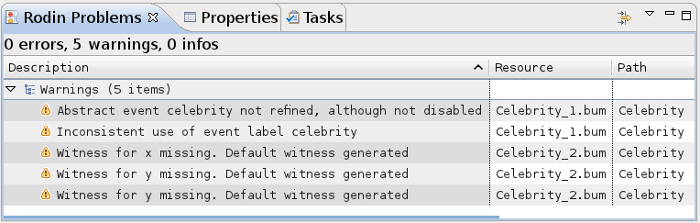
\includegraphics{img/tutorial/tut_08_rodin_problems.png}
\end{center}

In the first part of this section, our goal is to fix these problems. Let's take a look at the warning stating that the event label ``celebrity'' is misused (``Inconsistent use of event label celebrity	Celebrity''). Double-click on the warning to open the \texttt{Celebrity\_1} machine. The problem is that it is not declared as a refinement. Expand the event and add a new entry in the \textsf{REFINES} section (Click on the green plus-sign to create a new entry). Select the event \textsf{celebrity}. This declares that the event is a refinement of an event with the same name in the abstract machine (\ref{abstract_machine}). As this is the case here, we can now save the project and the warning disappears.

The three remaining warnings state that witnesses (\ref{witness}) are missing. In any abstract event that uses parameters, if the concrete event has no parameter with the same name, the tool needs a witness (\ref{witness}) so that it notices what value the parameter should take. Witnesses (\ref{witness}) are also needed for variables that have a non-deterministic (\ref{non_deterministric}) assignment in an abstract event and do not appear in the concrete model. To create the witness (\ref{witness}), double-click on the warning to open the concrete model (here \texttt{Celebrity\_2}). Then, expand the \textsf{celebrity} event and add a witness (\ref{witness}) in the \textsf{WITH} section (Click on the green plus-sign to create a new entry).

A default witness (\ref{witness}) \textsf{wit1} has been created, with a default value \textsf{$\top$} (e.g. the predicate ``true'') which we need to change. Its name will have to be \textsf{x} if we want it to be a witness (\ref{witness}) for the parameter \textsf{x} of the corresponding abstract event in the machine \texttt{Celebrity\_1}. The abstract event has the assignment \textsf{$r \bcmeq x$}, while the concrete one has the assignment \textsf{$r \bcmeq b$}. So the content of the witness is \textsf{x = b}. The event should now look as follows: 

\begin{description}
	\EVT {celebrity}
	\REF {celebrity}
		\begin{description}
		\WhenGrd
			\begin{description}
			\nItemX{ grd1 }{ R = \emptyset  }
			\end{description}
		\Witnesses
			\begin{description}
			\nItem{ x }{ x=b }
			\end{description}
		\ThenAct
			\begin{description}
			\nItemX{ act1 }{ r :=  b }
			\end{description}
		\EndAct
		\end{description}
\end{description}

Edit the content and save the file. One warning will disappear, two to go.

\info{
Try completing the other two witnesses on your own. A hint: Both witnesses are simple equalities, and both can be found by comparing the third guard of the abstract event with the second guard of the concrete one. Remember to give the witness the name of the variable it stands for. If you completed this step correctly, there should be no warning, info or error left on the Rodin Problems View (\ref{rodin_problems_view}).
}

The following section \ref{tut_08_final_celebrity} shows the final \texttt{Celebrity\_2} machine.

\subsection{The Final Second Refinement} \label{tut_08_final_celebrity}

TODO: add event-b spec

\subsection{The Proving Perspective}

In this section we prove the model of the Celebrity Problem. Therefore, switch to the Proving Perspective. You can switch between perspectives using the shortcut bar: 

\begin{center}
	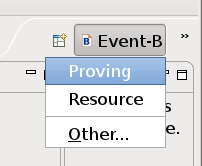
\includegraphics{img/tutorial/tut_08_switch_perspective.png}
\end{center}

\warning{If the Proving Perspective is not available in the menu, select \textsf{Other... $\rangle$ Proving}. This will open a new window which shows all available Perspectives.}

We should now see the following window: 

TODO: make a new screenshot with the Celebritiy project in the explorer

\begin{center}
	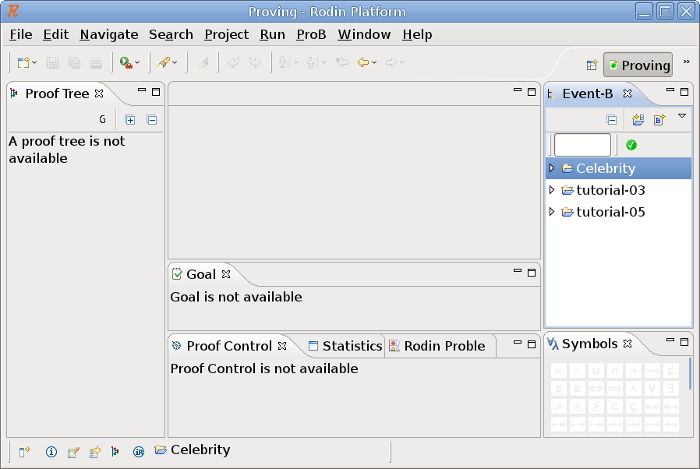
\includegraphics{img/tutorial/tut_08_proving_perspective.png}
\end{center}

The Proving Perspective contain three new views:

\begin{description}
	\item[Proof Tree View (\ref{proof_tree_view})] Here we see a tree of the proof that we have done so far and the current position in it. By clicking in the tree, we can navigate inside the proof. Currently, we have not started with the proof yet, so there is no new place to move to. 
	\item[Proof Control View (\ref{proof_control_view})] This is where we perform interactive proofs.
	\item[Goal View (\ref{goal_view})] This window shows what needs to be proved at the current position inside the proof tree.
\end{description}

Browsing around in the Event-B Explorer (\ref{eventb_explorer}), we can see that the auto-prover (\ref{auto_prover}) did quite a good job. All except for three proofs already should be completed. Except for the last one of them, all of them could be proved with a different external prover, but in order to learn a few new techniques, we will prove them with the so called ``p0 prover'' (\ref{p0_prover}).

Let's start with the proof \textsf{remove\_1/inv2/INV} of \texttt{Celebrity\_1}. For this expand the \texttt{Celebrity\_1} machine in the Event-B Explorer (\ref{eventb_explorer}), expand the Proof Obligations (\ref{proof_obligation}) and double-click on \textsf{remove\_1/inv2/INV}:

\begin{center}
	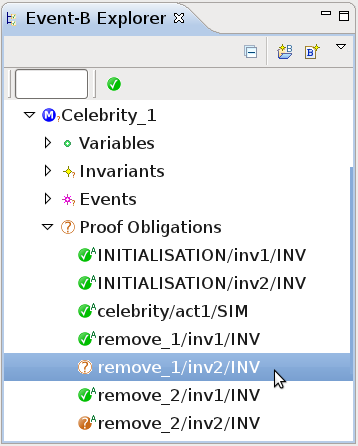
\includegraphics{img/tutorial/tut_08_proof1.png}
\end{center}

We should now see the following window:

\begin{center}
	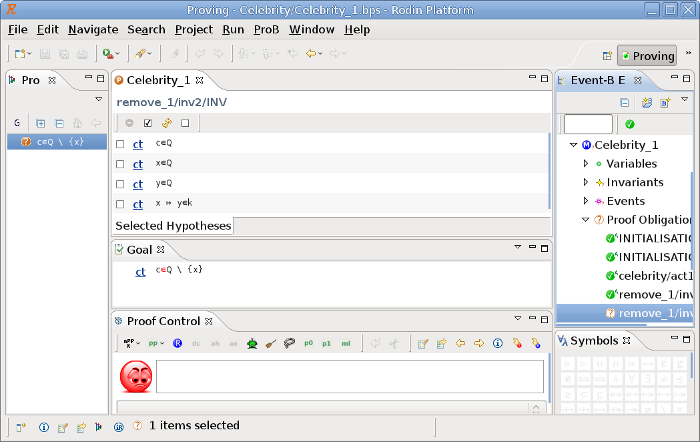
\includegraphics{img/tutorial/tut_08_proof2.png}
\end{center}


TODO: change or improve explanations because there is a lack of advices (example: use lasso button and click on p1)

In order to prove the statement, it suffices to prove \textsf{$x \neq c$}. So type this into the \textsf{Proof Control View} (\ref{proof_control_view}) and press the ah \textsf{Add Hypothesis button (ah)}. Now, press \textsf{p0} until it does not get you any further. Now, try selecting the right hypotheses by yourself in order to complete the proof. If you cannot find it, you may also just select all hypotheses.

In order to move to the next Proof Obligation (\ref{proof_obligation}), you may also use the \textsf{Next Undischarged PO button (The small right arrow icon)} of the \textsf{Proof Control View} (\ref{proof_control_view}). The next proof can be solved the same way as the last one.

\info{As an exercise, try to prove \texttt{Celebrity\_2}. A small hint: We have to fill in an existential quantifier. First, look in the list of hypothesis if you find any variable that is in P, and select that hypothesis. Then, instantiate \textsf{b'} and \textsf{R'} correctly (For instance, if you want to instantiate \textsf{b'} with \textsf{c}, then \textsf{$P \backslash \{ c\}$} is a good choice for \textsf{R'}) by typing the instantiations in the \textsf{Goal View} (\ref{goal_view}) and then clicking on the red existential quantifier. Now, all open branches of the proof tree can be proved with \textsf{p0}. After this, we have completed all the proofs, and the model is ready for use. } 
